\clearpage
\setcounter{page}{1}

\section{Tutorial membuat aplikasi oracle apex}
\begin{enumerate}
    \item Langkah pertama, buka oracle apex online \textit{oracle.apex.com}. Untuk yang belum memiliki akun anda bisa memilih get started for free dan bagi anda yang sudah memiliki akun anda bisa langsung sign in.
        \begin{figure}[h]
        \centerline{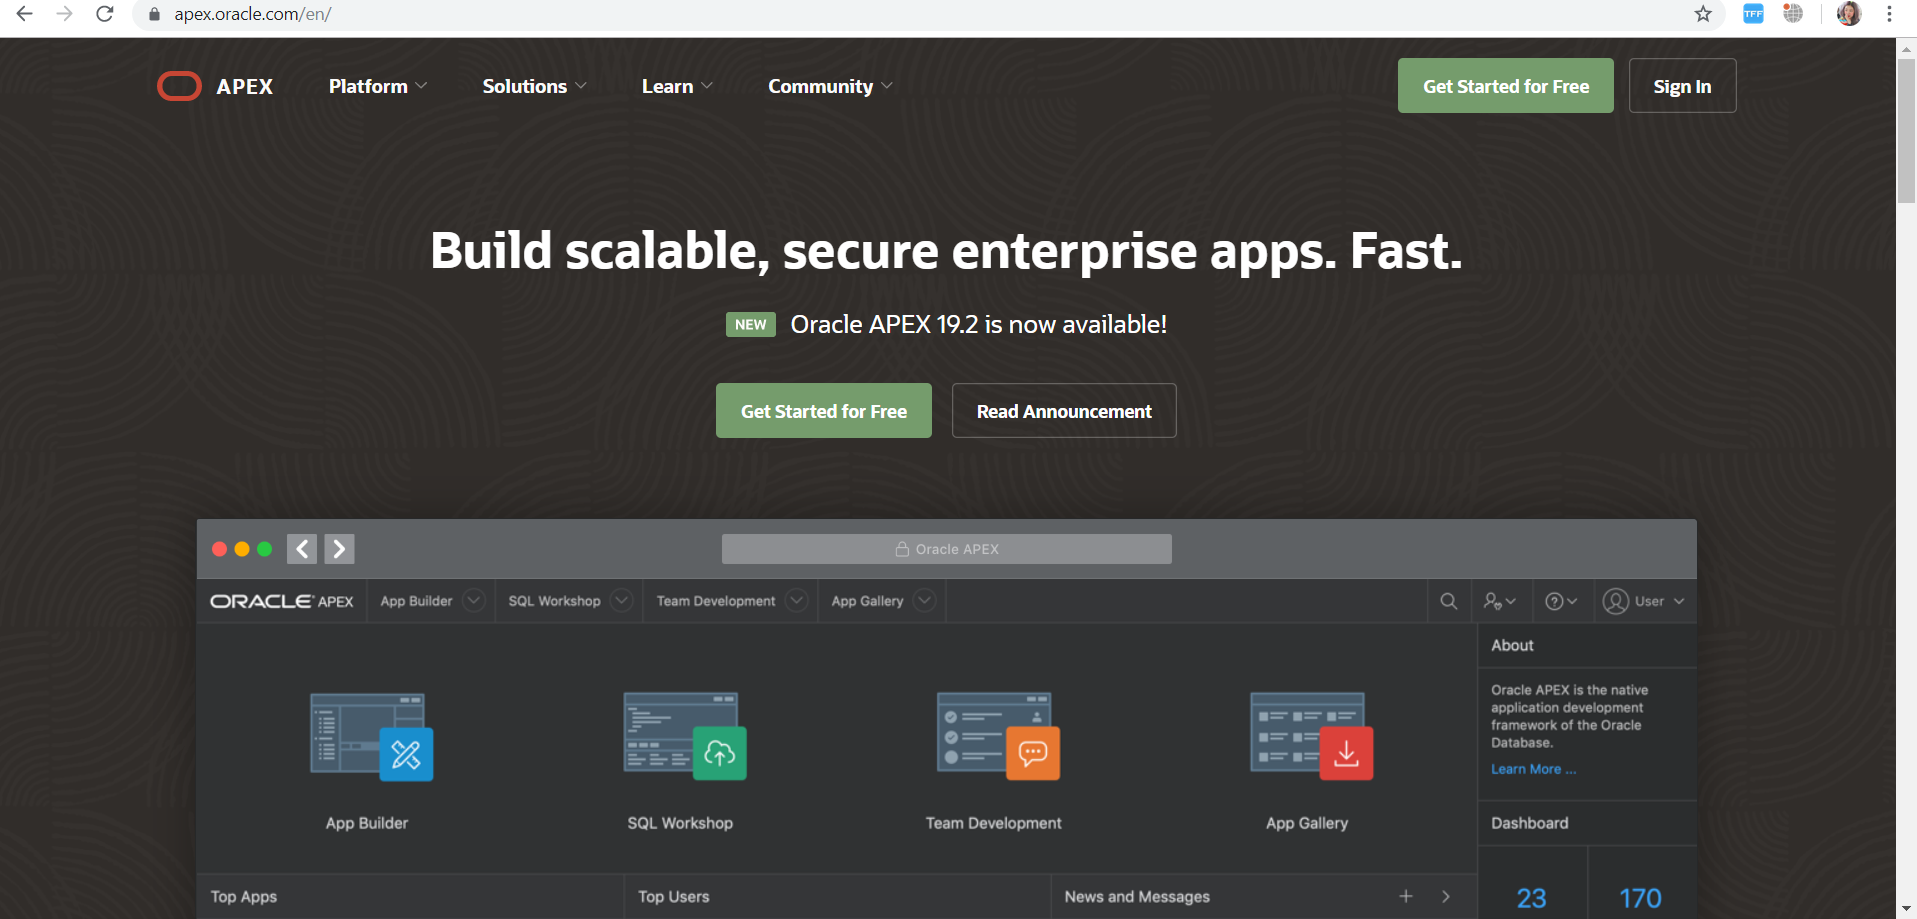
\includegraphics[width=8cm]{GAMBAR/getstarted.PNG}}
        \end{figure}
    \item Berikut adalah tampilan setelah mengklik get started for free, klik request for a workspace dan ikuti langkah selanjutnya dengan mengisi data diri anda.
        \begin{figure}[h]
        \centerline{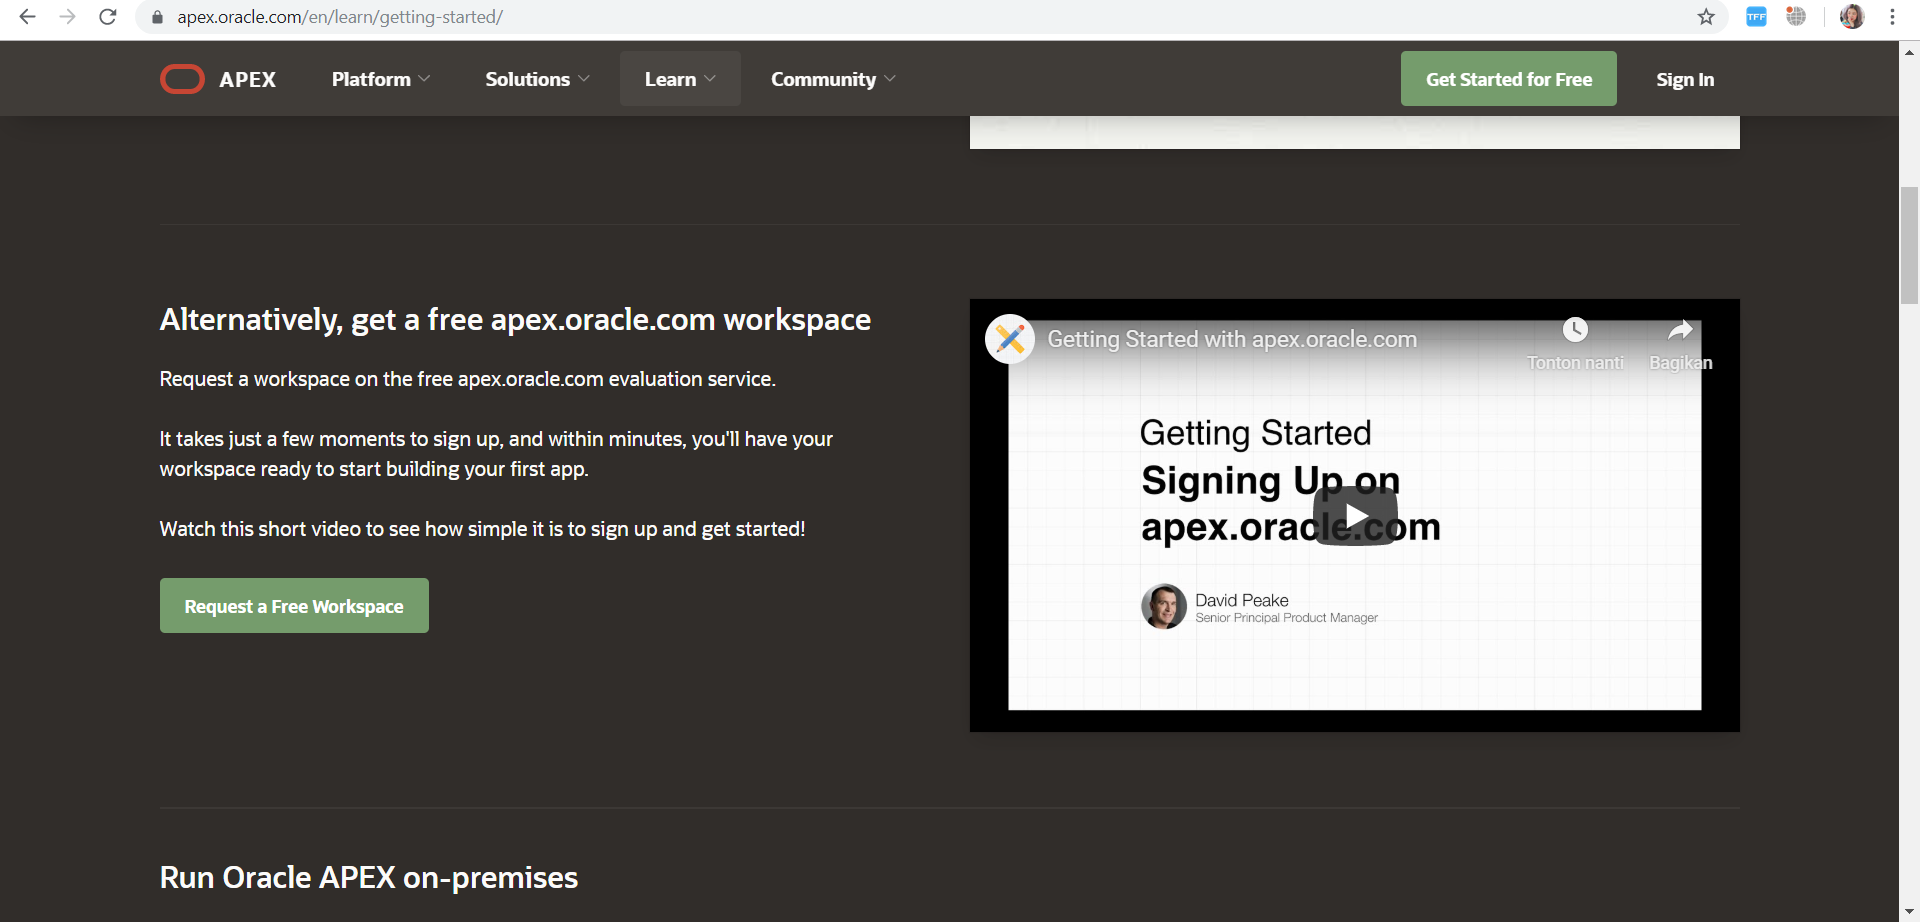
\includegraphics[width=8cm]{GAMBAR/requestws.PNG}}
        \end{figure}
    \item Selanjutnya adalah tampilan untuk Sign In, silahkan isi workspace, username, dan password yang anda miliki.
        \begin{figure}[h]
        \centerline{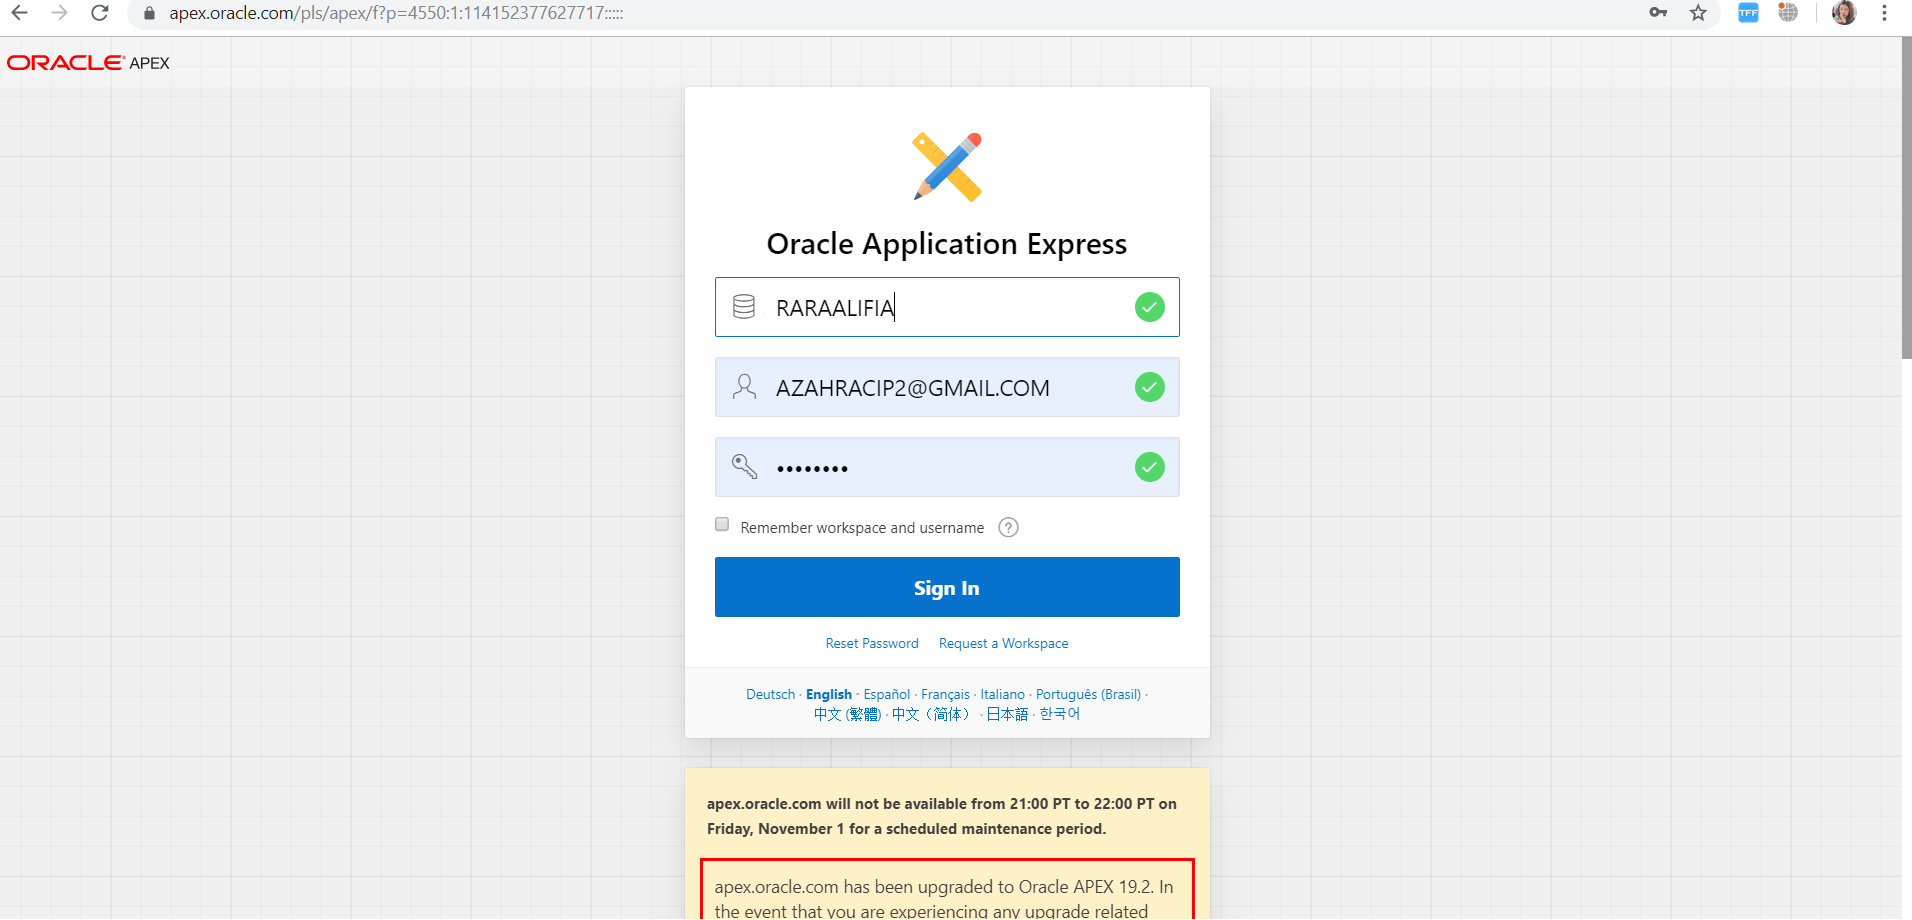
\includegraphics[width=8cm]{GAMBAR/SIGNIN2.PNG}}
        \end{figure}
    \item Lalu klik app builder
        \paragraph{}
        \centerline{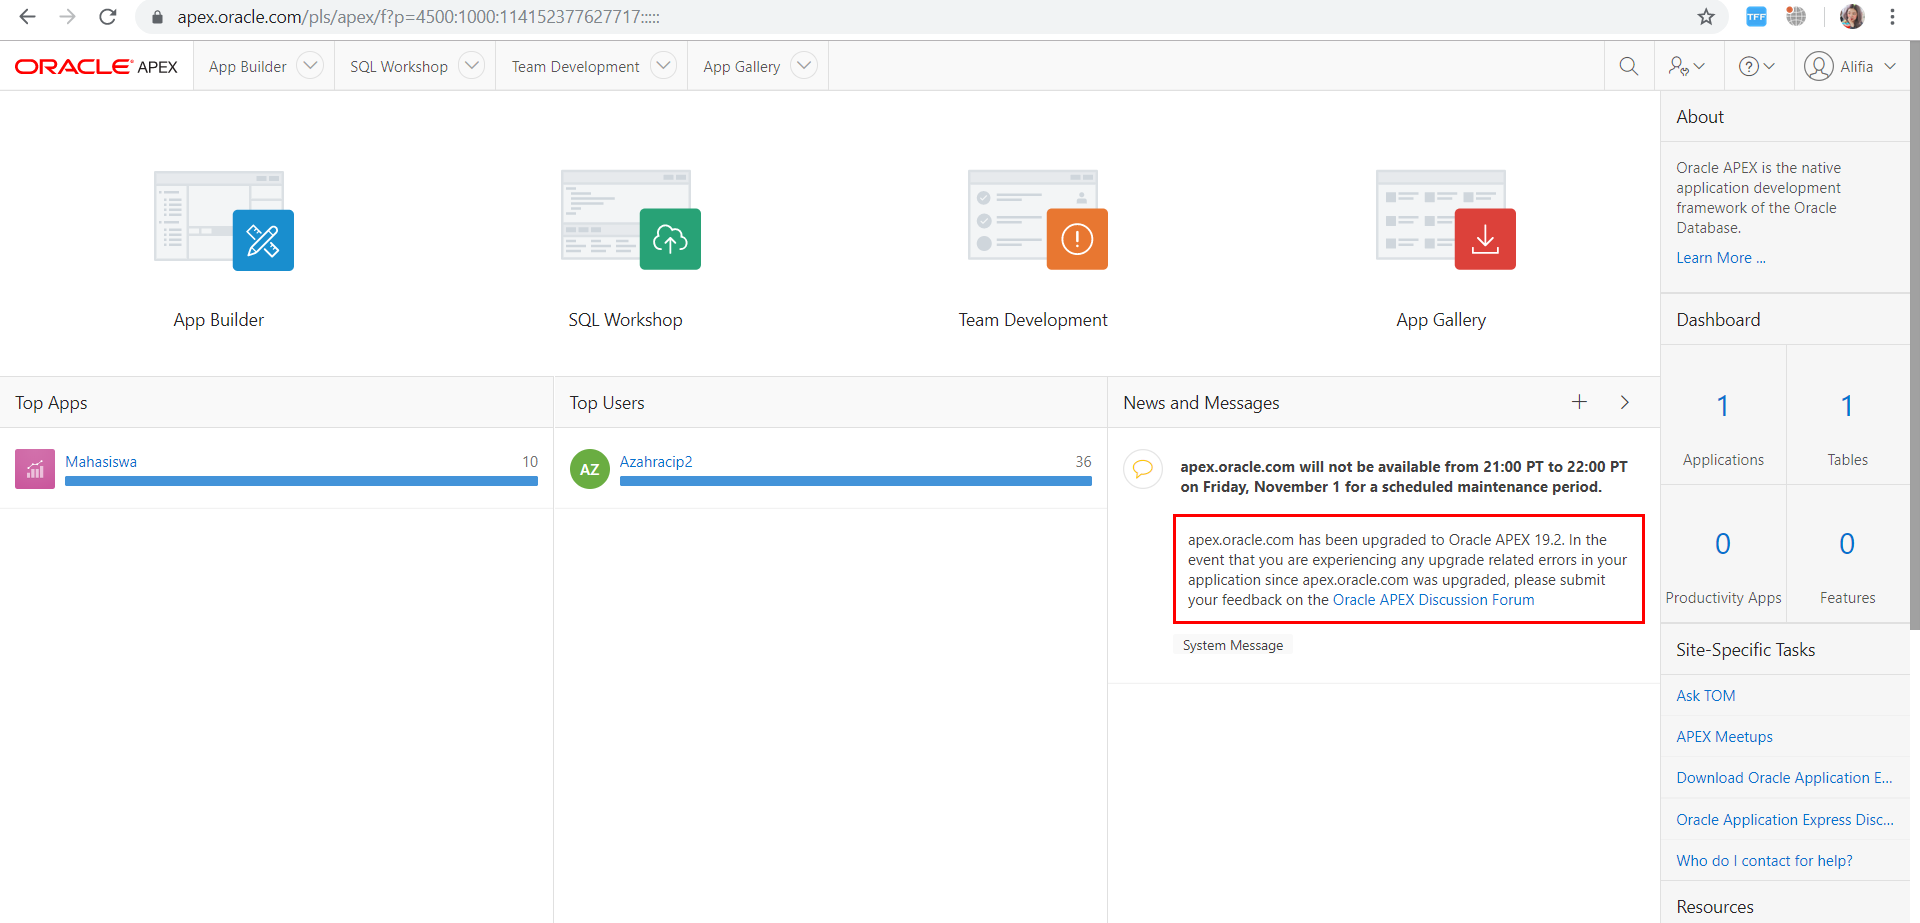
\includegraphics[width=8cm]{GAMBAR/APPBUILDER.PNG}}
    \item Klik create untuk membuat aplikasi
        \begin{figure}[h]
        \centerline{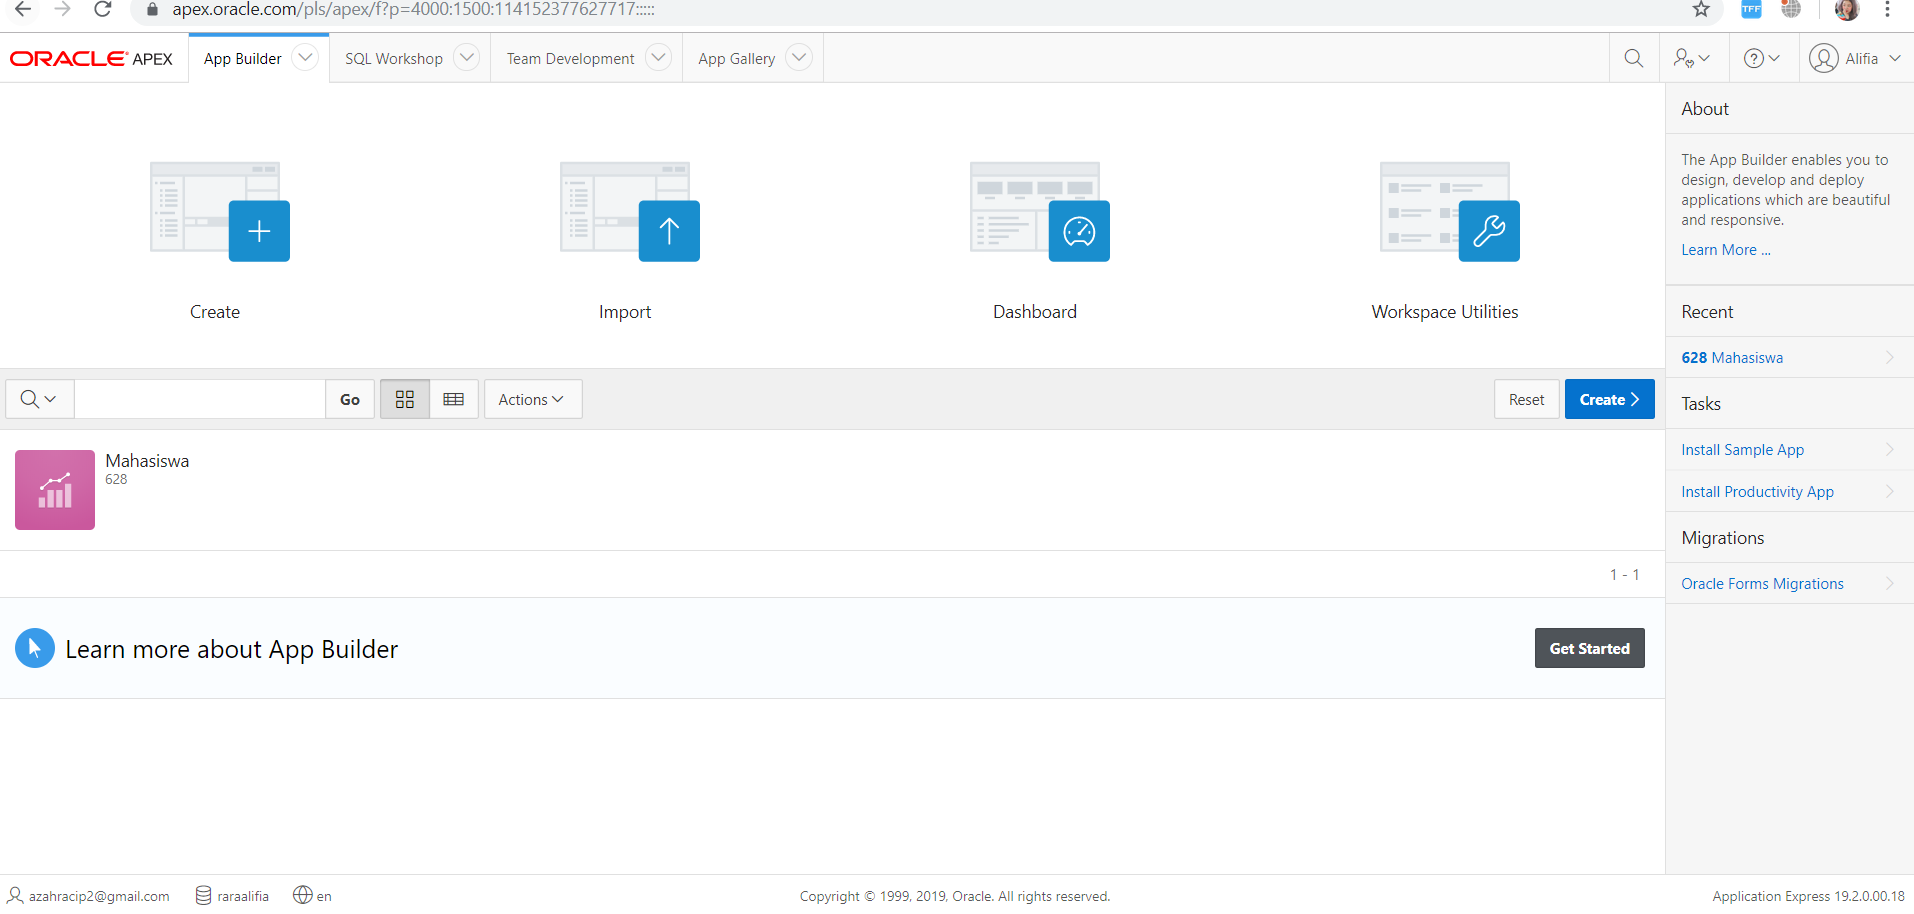
\includegraphics[width=8cm]{GAMBAR/CREATE.PNG}}
        \end{figure}
    \item Pilih opsi from a file lalu upload file yang akan anda masukkan dalam aplikasi anda, pastikan ekstensinya \textit{csv.}
        \begin{figure}[h]
        \centerline{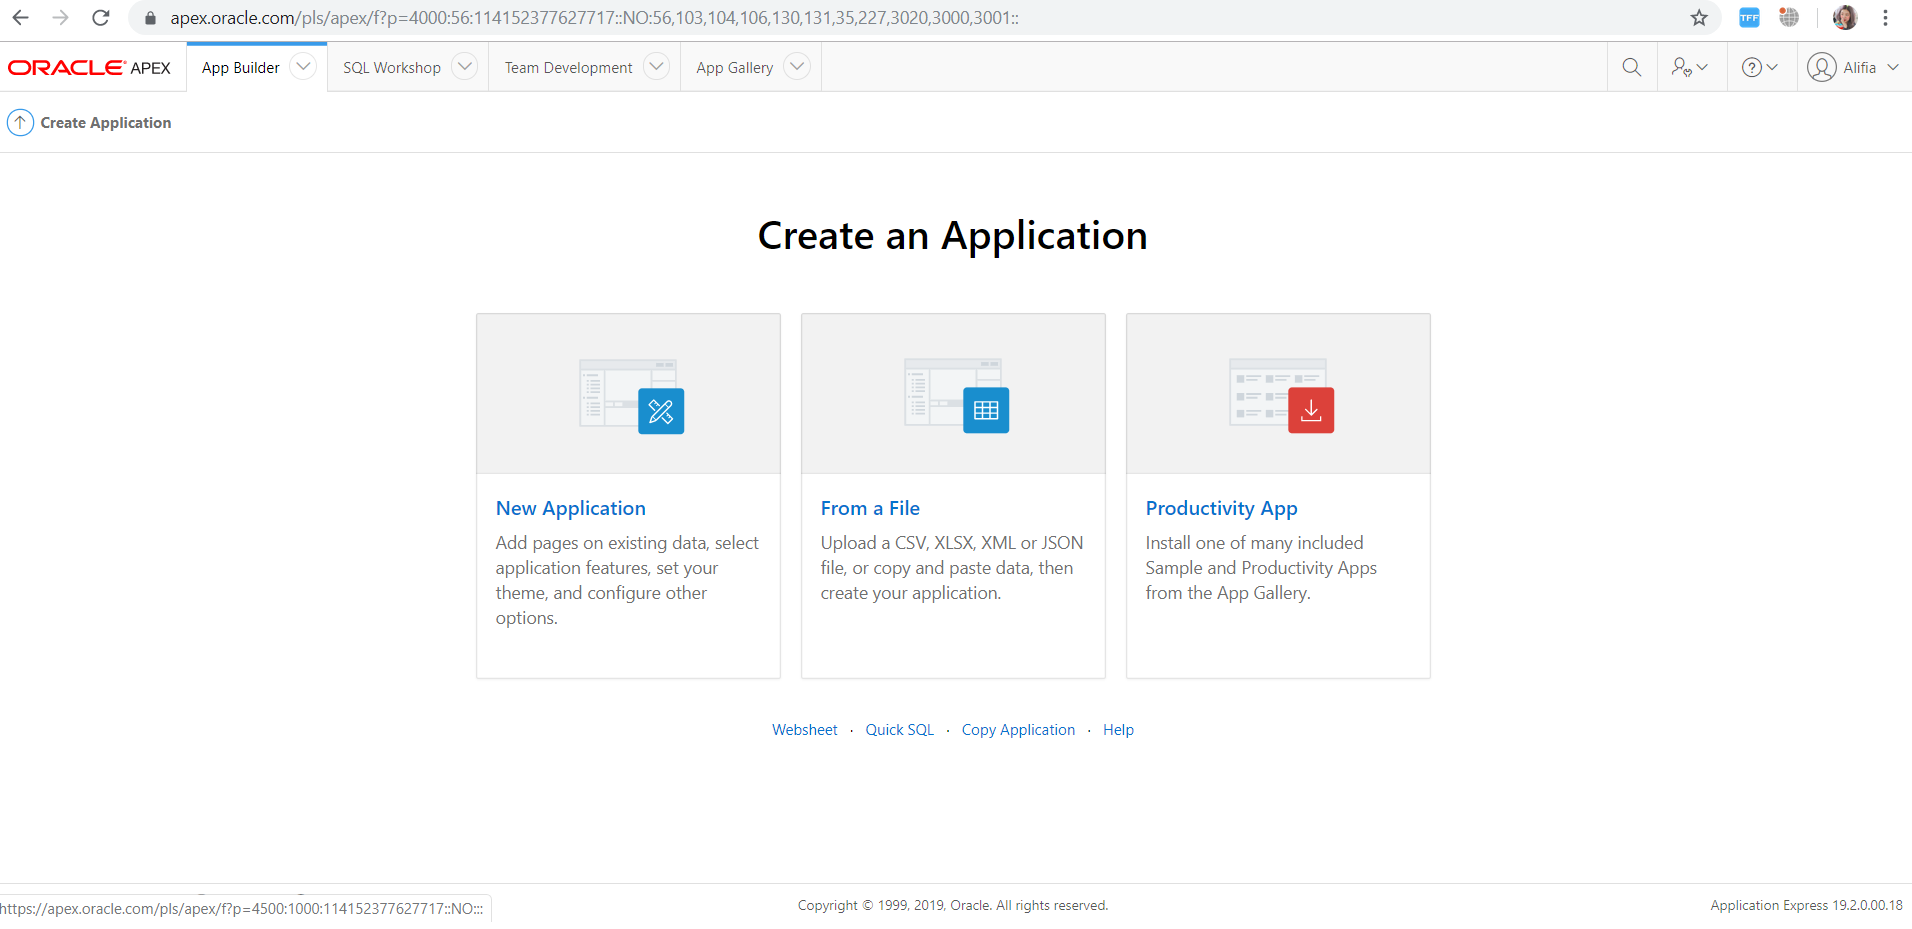
\includegraphics[width=8cm]{GAMBAR/FROMAFILE.PNG}}
        \end{figure}
        \begin{figure}[h]
        \centerline{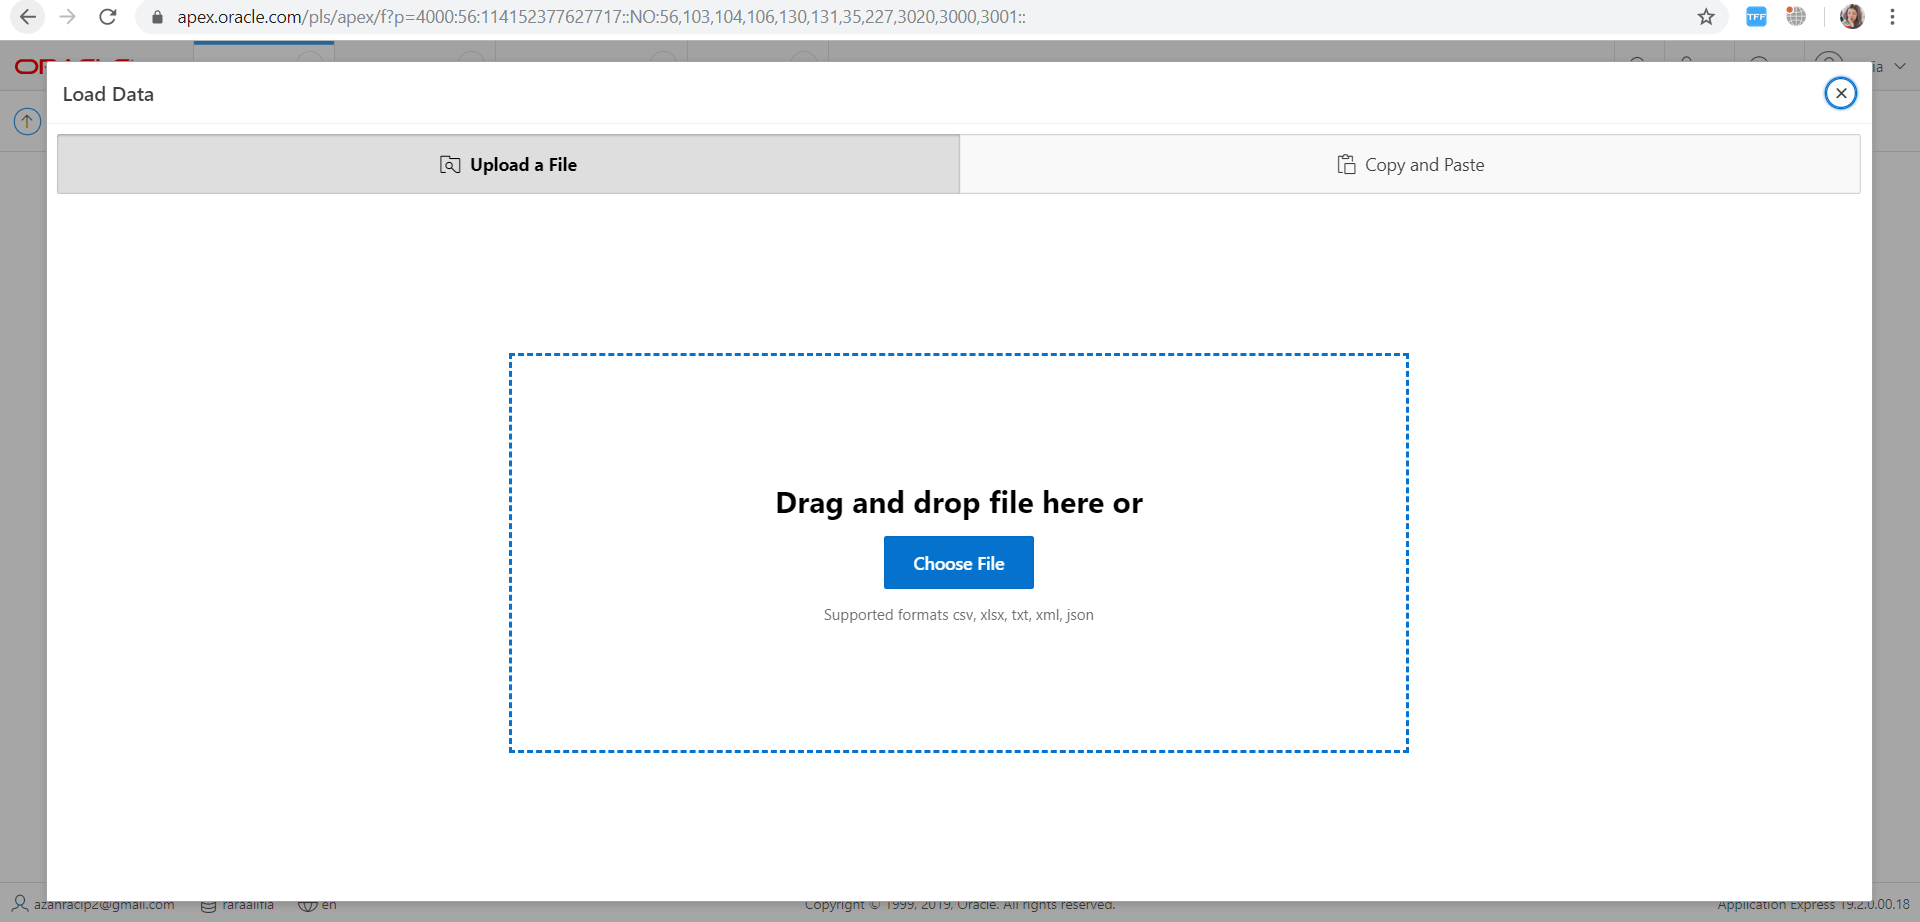
\includegraphics[width=8cm]{GAMBAR/CHOOSEFILE.PNG}}
        \end{figure}
    \item Disini saya akan mengupload file mahasiswad4ti, tabel prodi, tabel tingkat, dan tabel angkatan. Dimulai dari file yang kecil terlebih dahulu.
        \paragraph{}
        \centerline{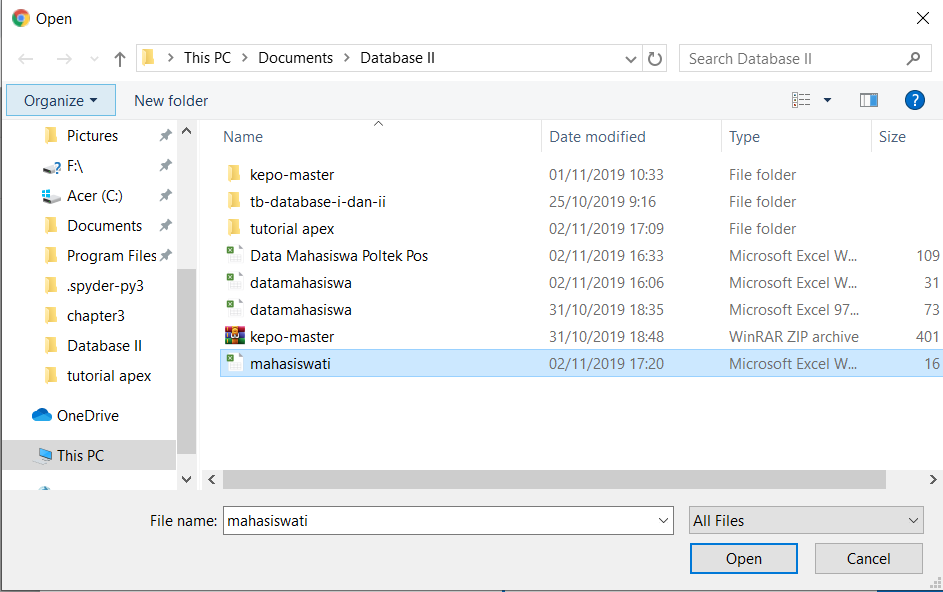
\includegraphics[width=8cm]{GAMBAR/DATAMHSTI.PNG}}
    \item Setelah itu isi table name sesuai keinginan anda, disini saya menamakan MAHASISWATI tetapi saya ubah menjadi MAHASISWA2, lalu klik configure.
        \begin{figure}[h]
        \centerline{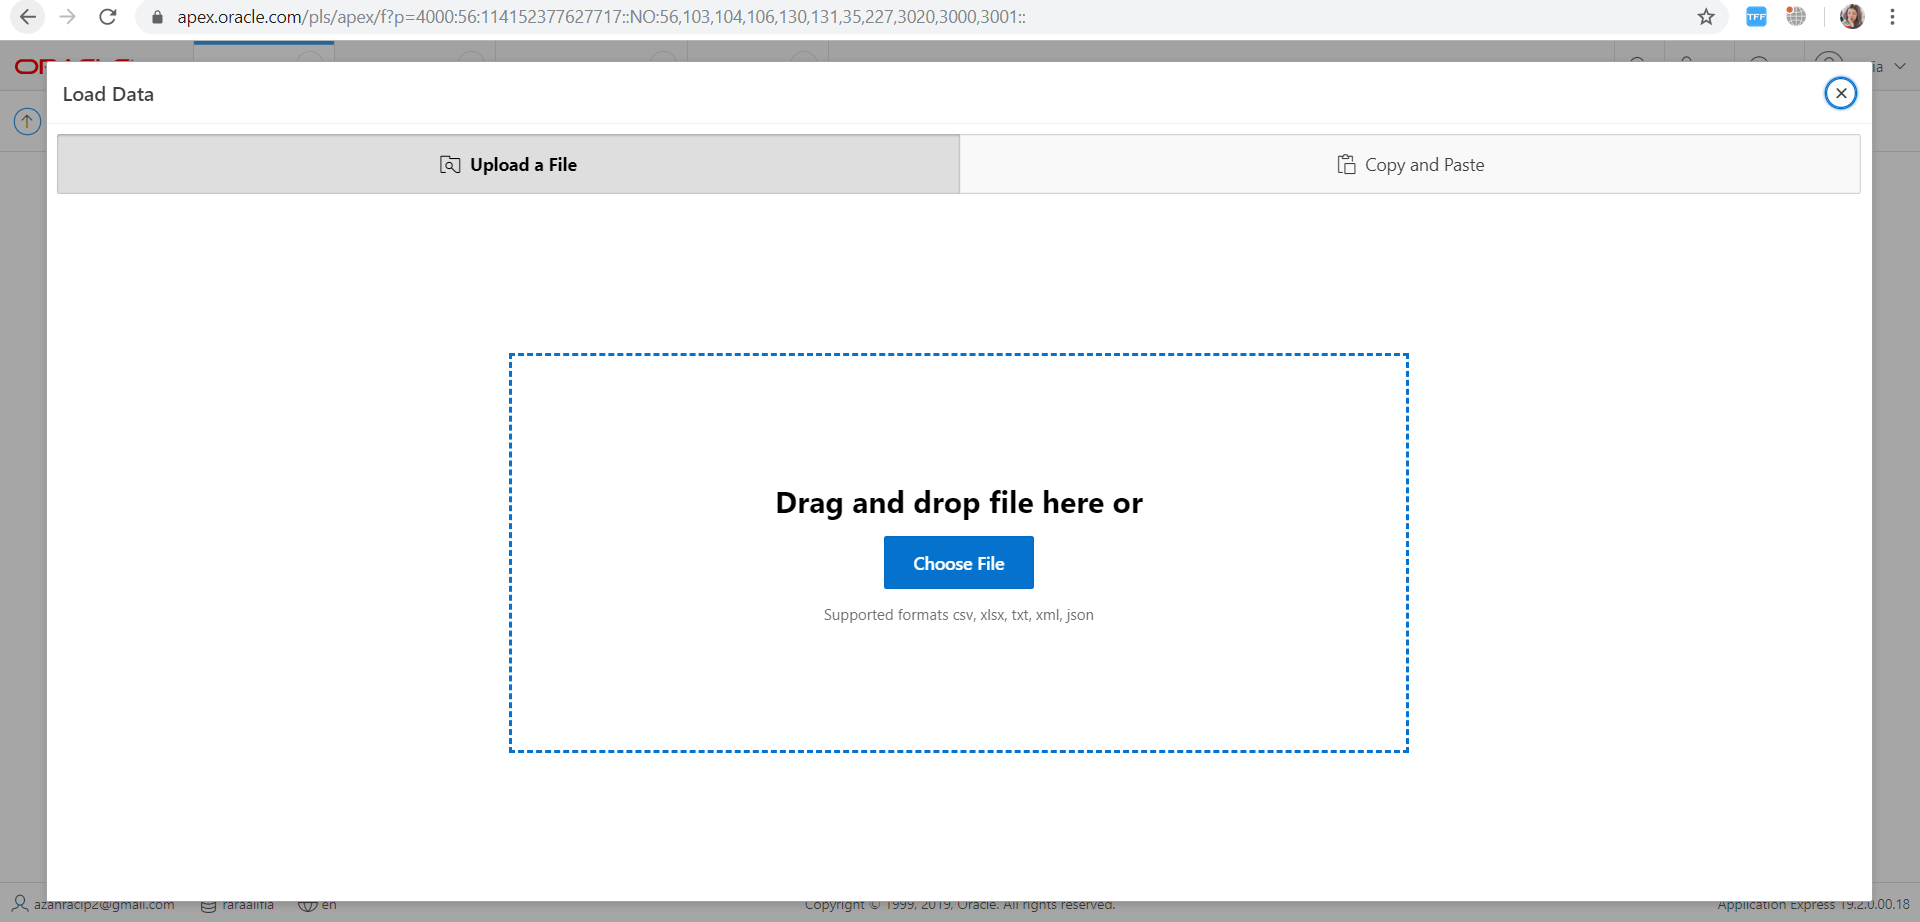
\includegraphics[width=8cm]{GAMBAR/CHOOSEFILE.PNG}}
        \end{figure}
    \item Klik Save Changes
        \begin{figure}[h]
        \centerline{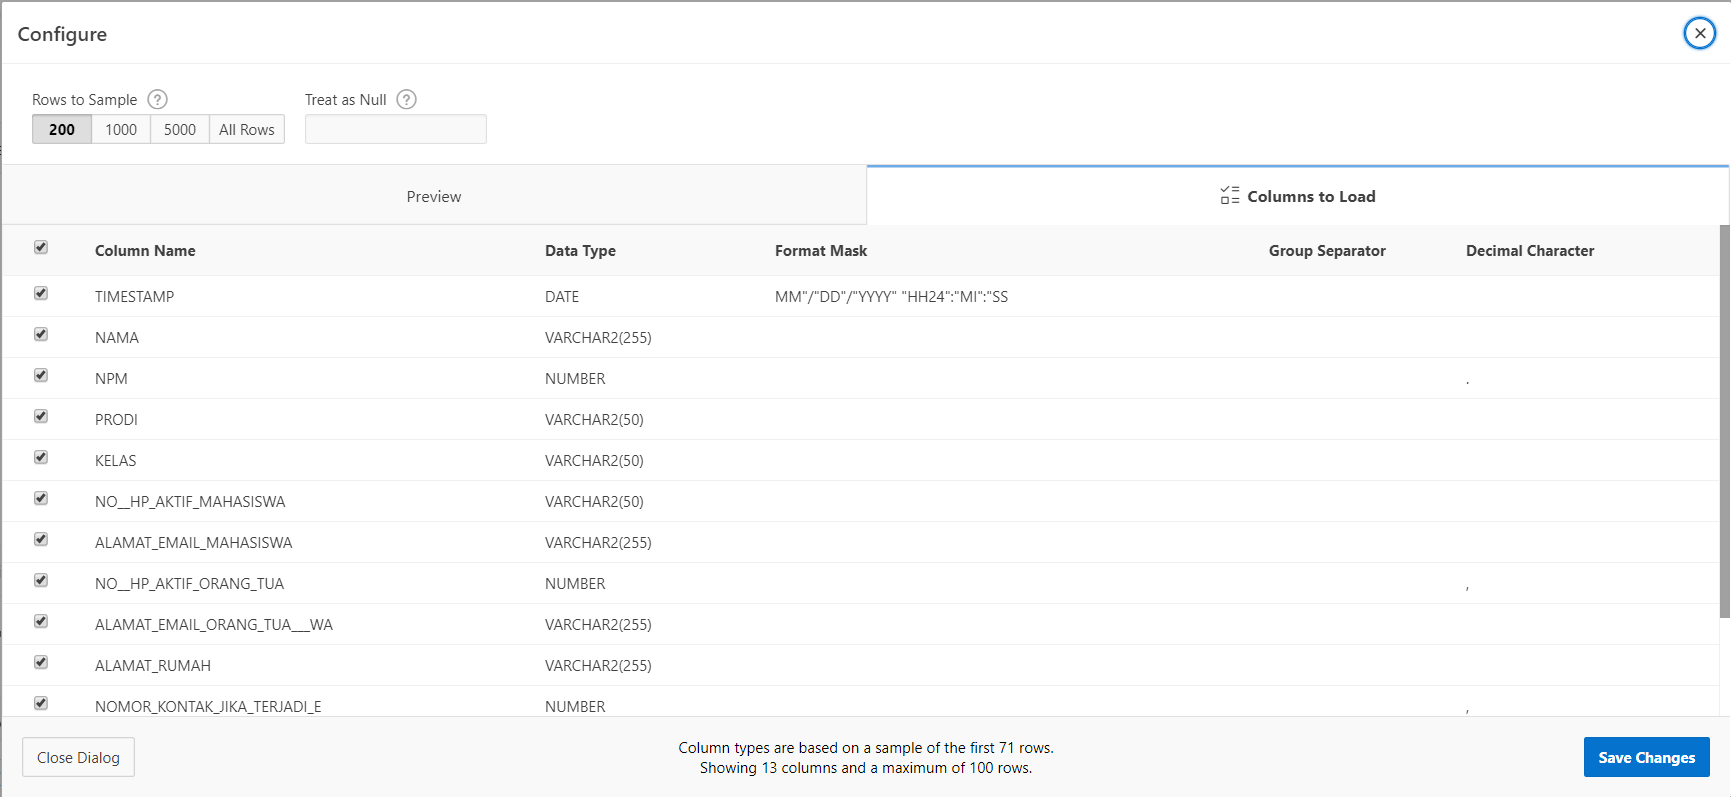
\includegraphics[width=8cm]{GAMBAR/CONFIG.PNG}}
        \end{figure}
    \item Klik load, lalu close dan ulangi langkah ke-6 untuk mengupload file anda yang lain.
        \paragraph{}
        \centerline{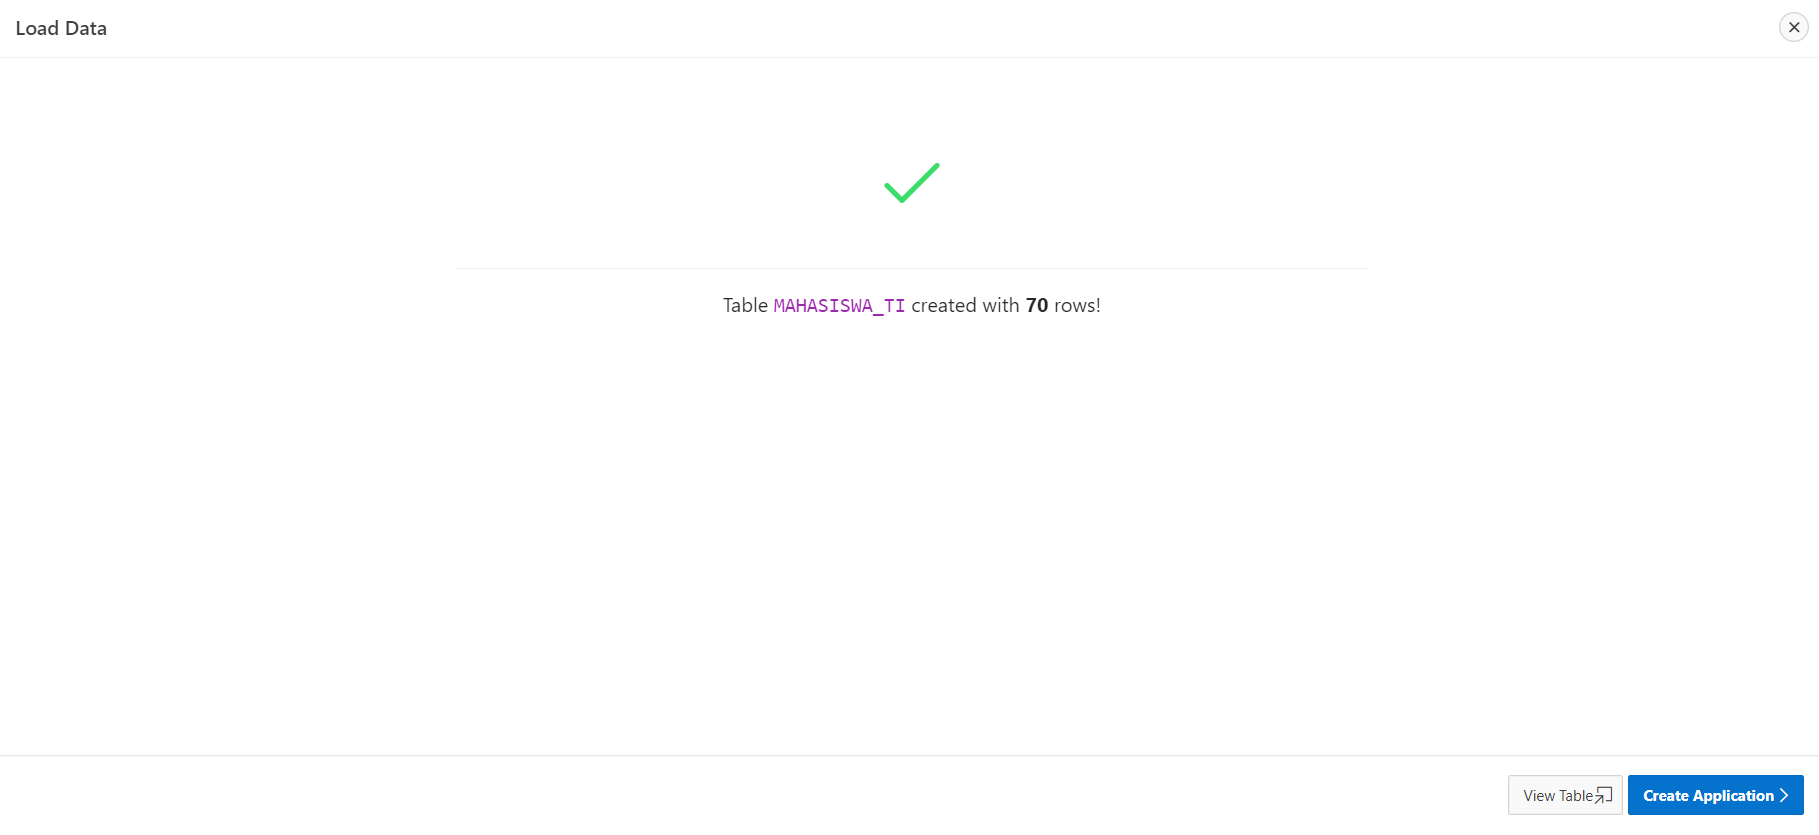
\includegraphics[width=8cm]{GAMBAR/VIEWTABLE.PNG}}
    \item Setelah file terupload semua, edit dan relasikan seperti berikut ini. Lalu blok satu persatu perintah dan run. 
        \begin{figure}[h]
        \centerline{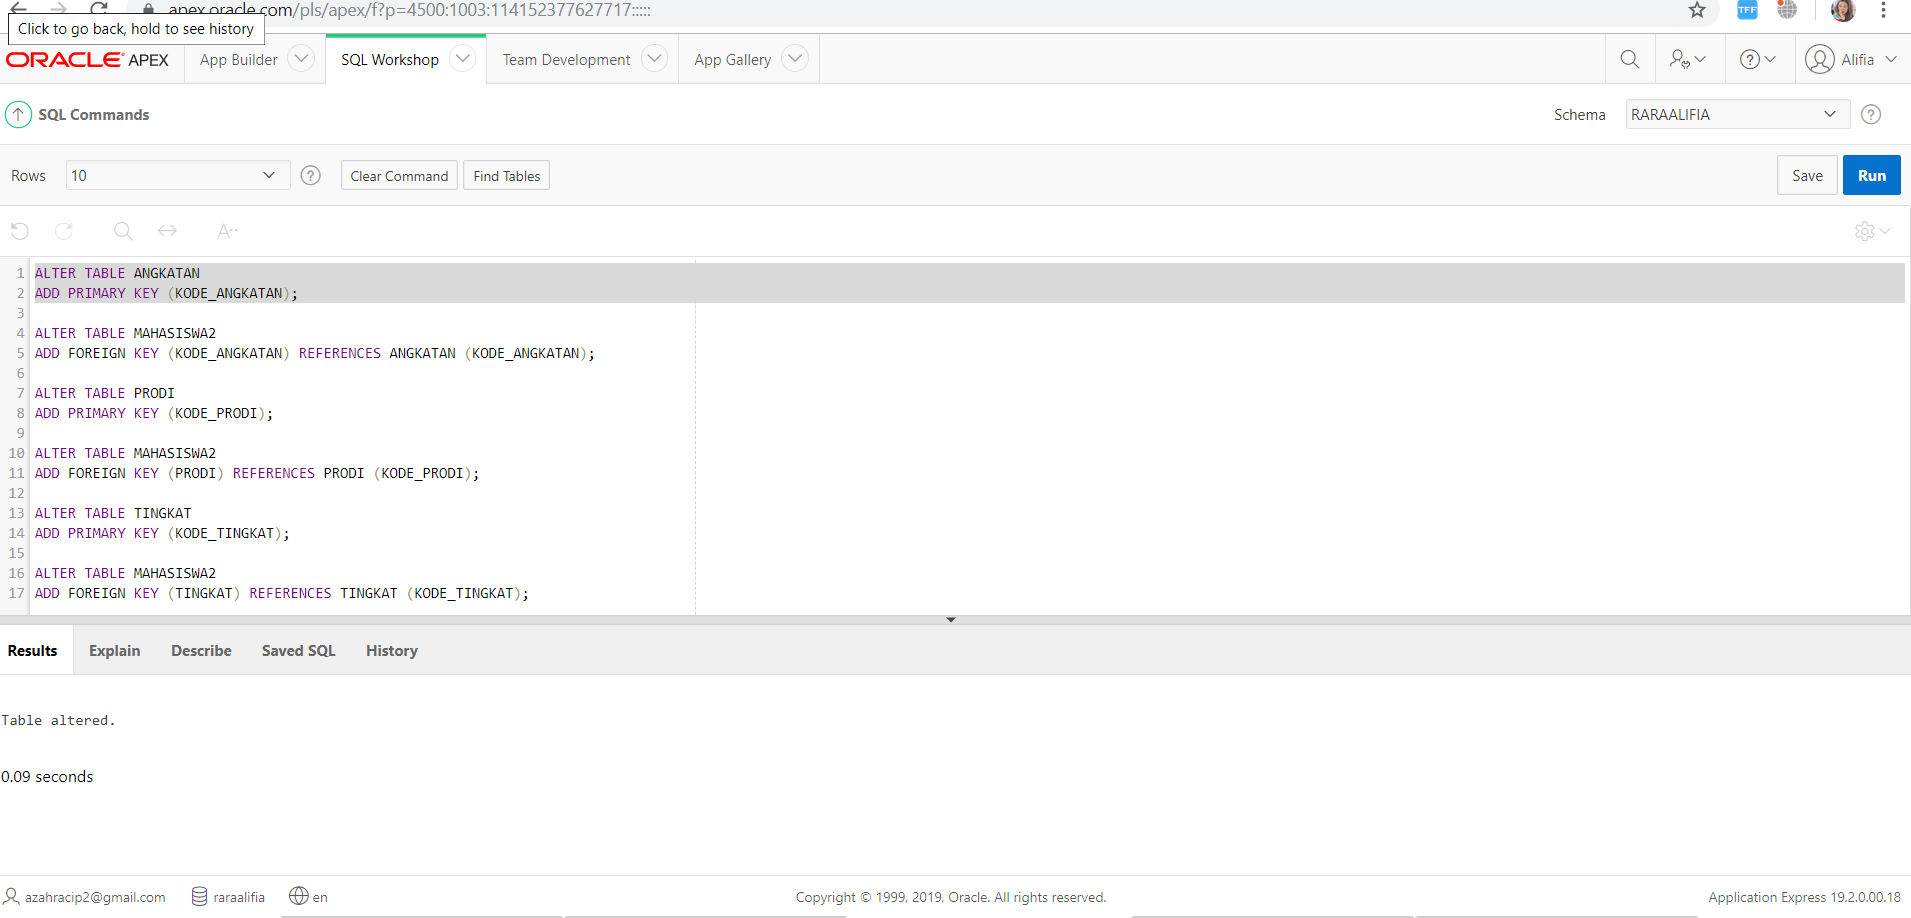
\includegraphics[width=8cm]{GAMBAR/COMMAND.PNG}}
        \end{figure}
    \item Lalu kembali ke app builder kemudian klik create lagi.
        \begin{figure}[h]
        \centerline{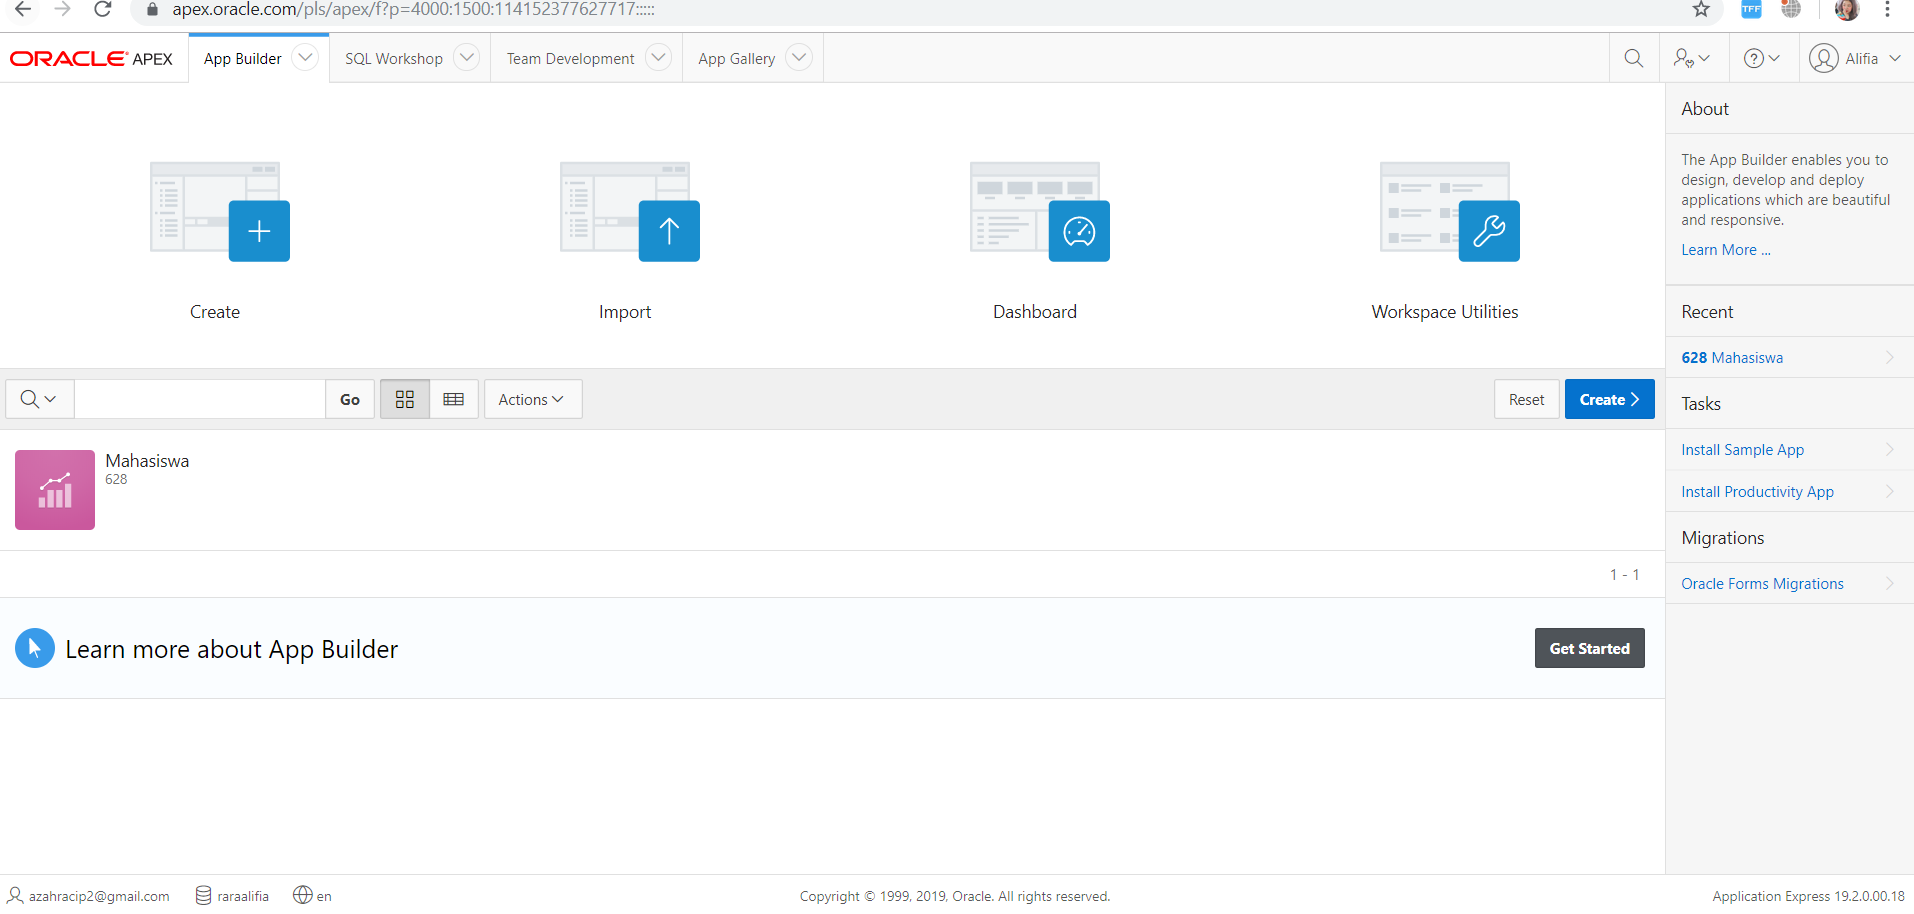
\includegraphics[width=8cm]{GAMBAR/CREATE.PNG}}
        \end{figure}
    \item Klik new application untuk membuat aplikasi baru
        \begin{figure}[h]
        \centerline{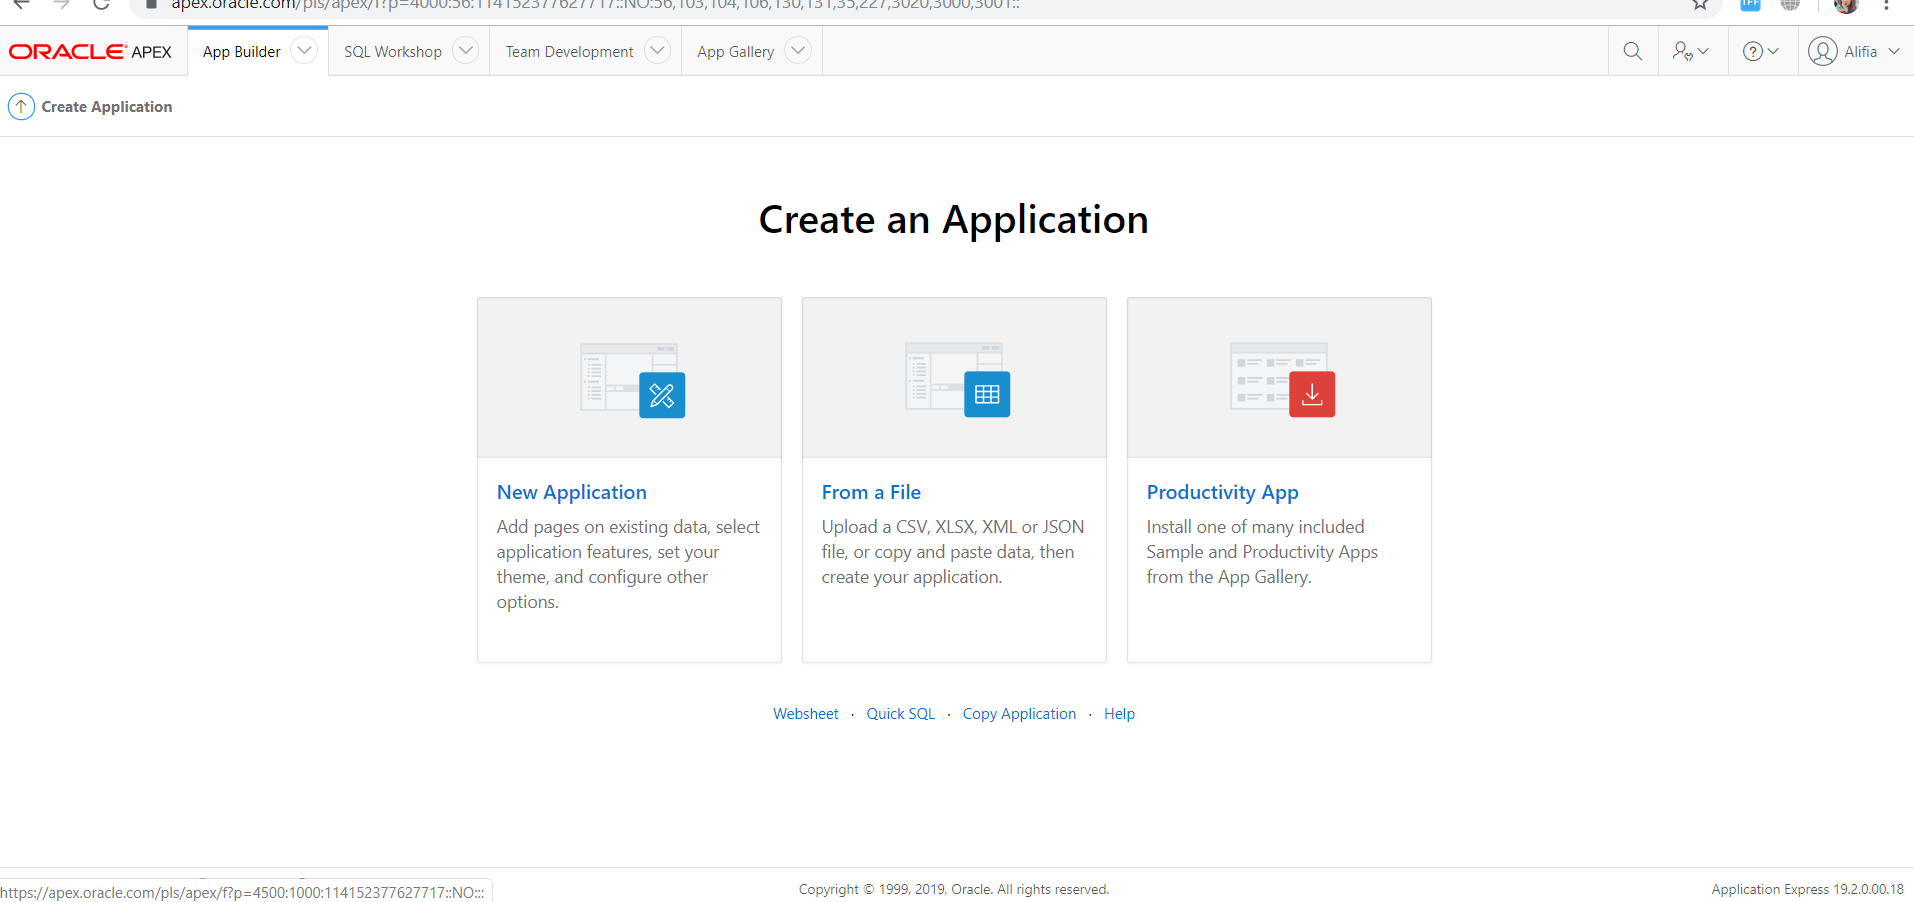
\includegraphics[width=8cm]{GAMBAR/NEWAPP.PNG}}
        \end{figure}
    \item Isi nama aplikasi sesuai keinginan anda
        \paragraph{}
        \centerline{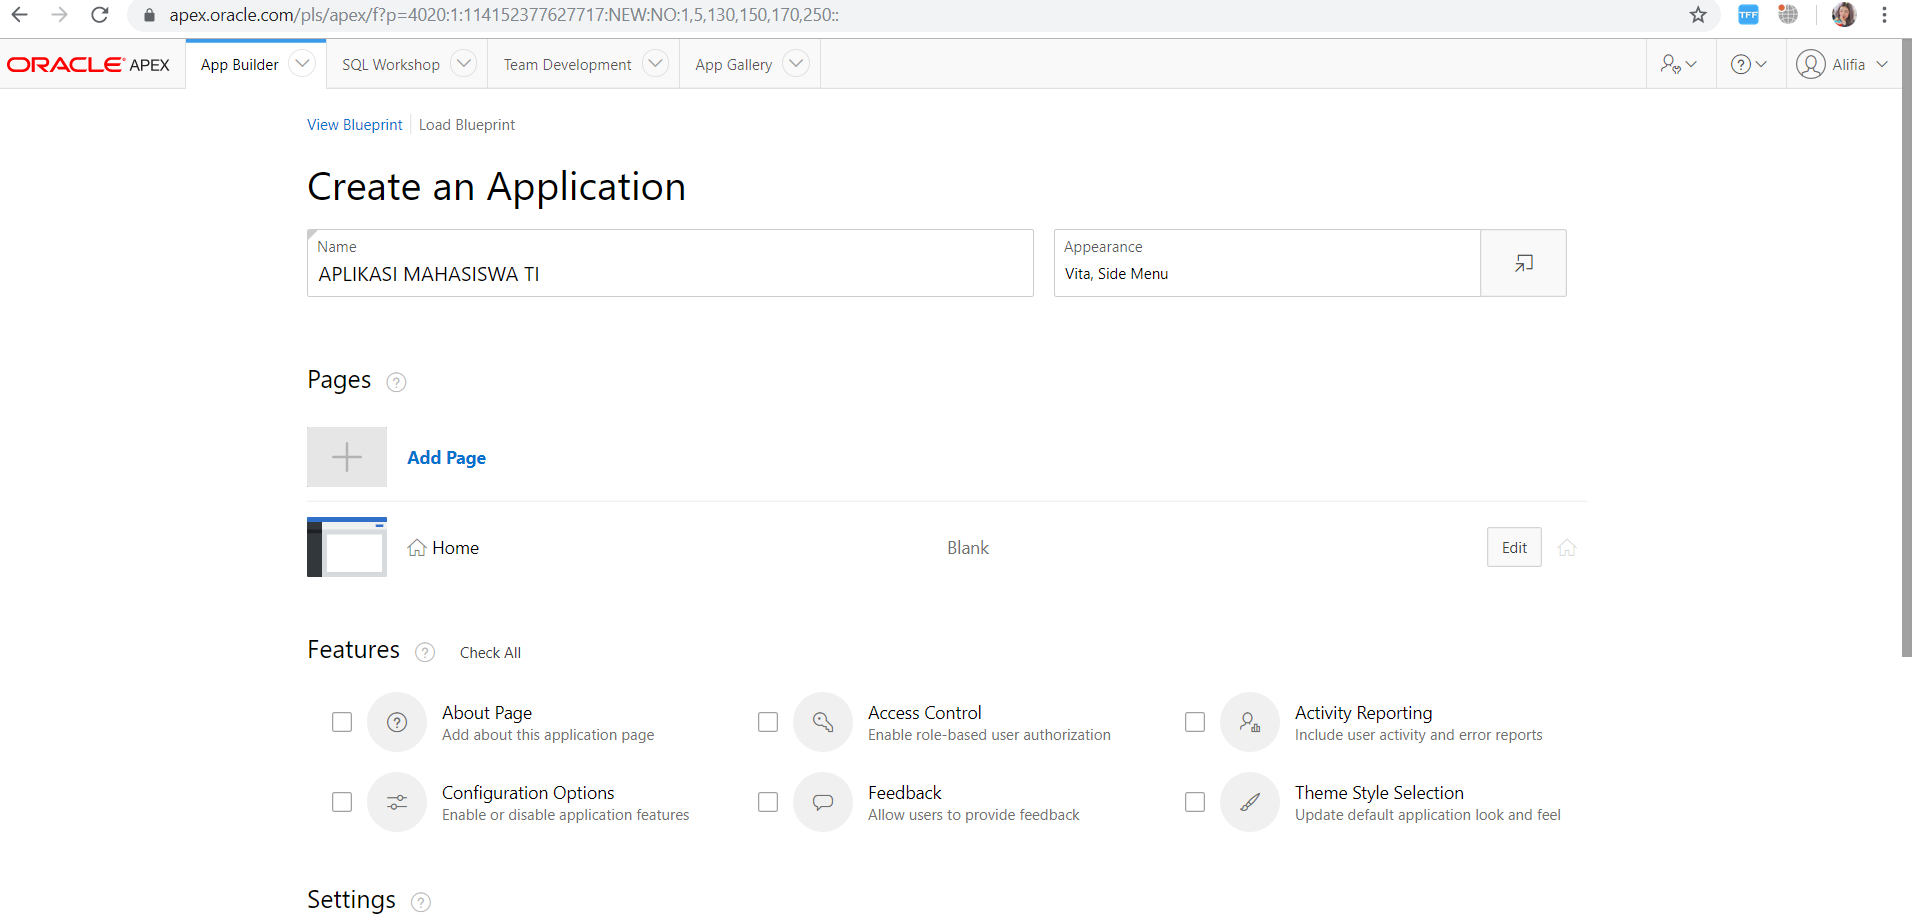
\includegraphics[width=8cm]{GAMBAR/APPMHSTI.PNG}}
    \item Langkah selanjutnya add page, kemudian pilih faceted search. Kemudian pilih add page lagi lalu pilih interactive report. Lalu create application.
        \begin{figure}[h]
        \centerline{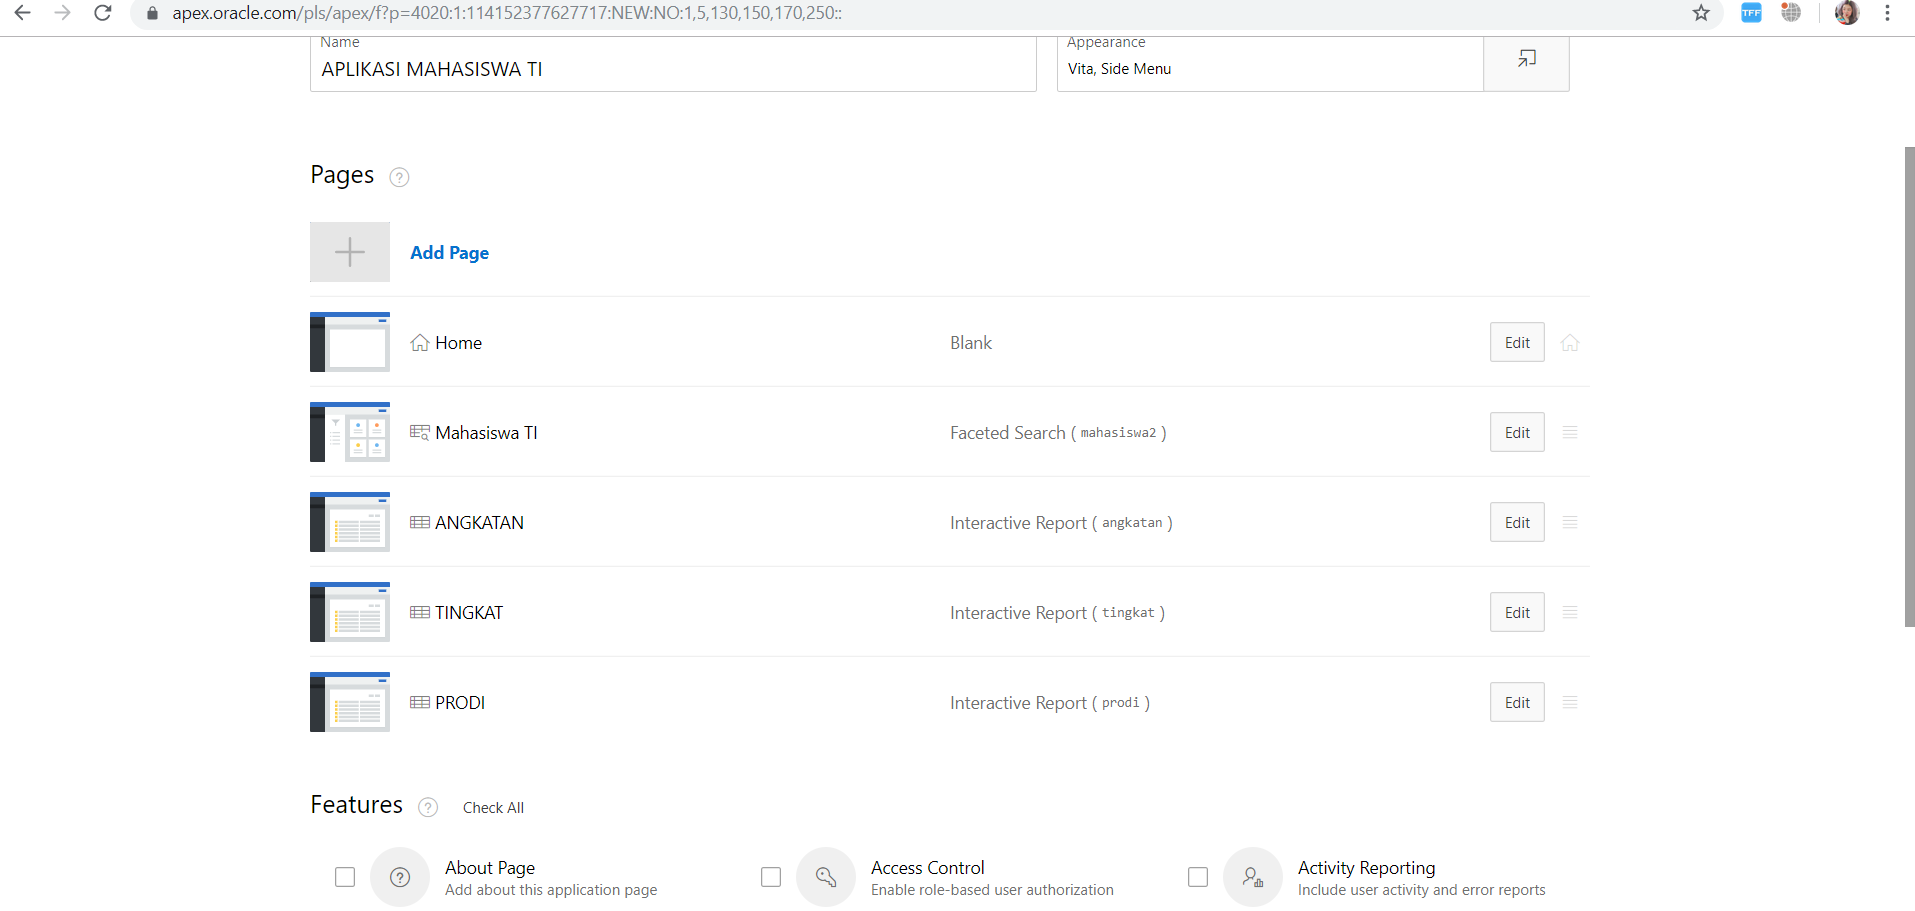
\includegraphics[width=8cm]{GAMBAR/ADDPAGE.PNG}}
        \end{figure}
    \item Lalu run application dan sign in kembali,
        \begin{figure}[h]
        \centerline{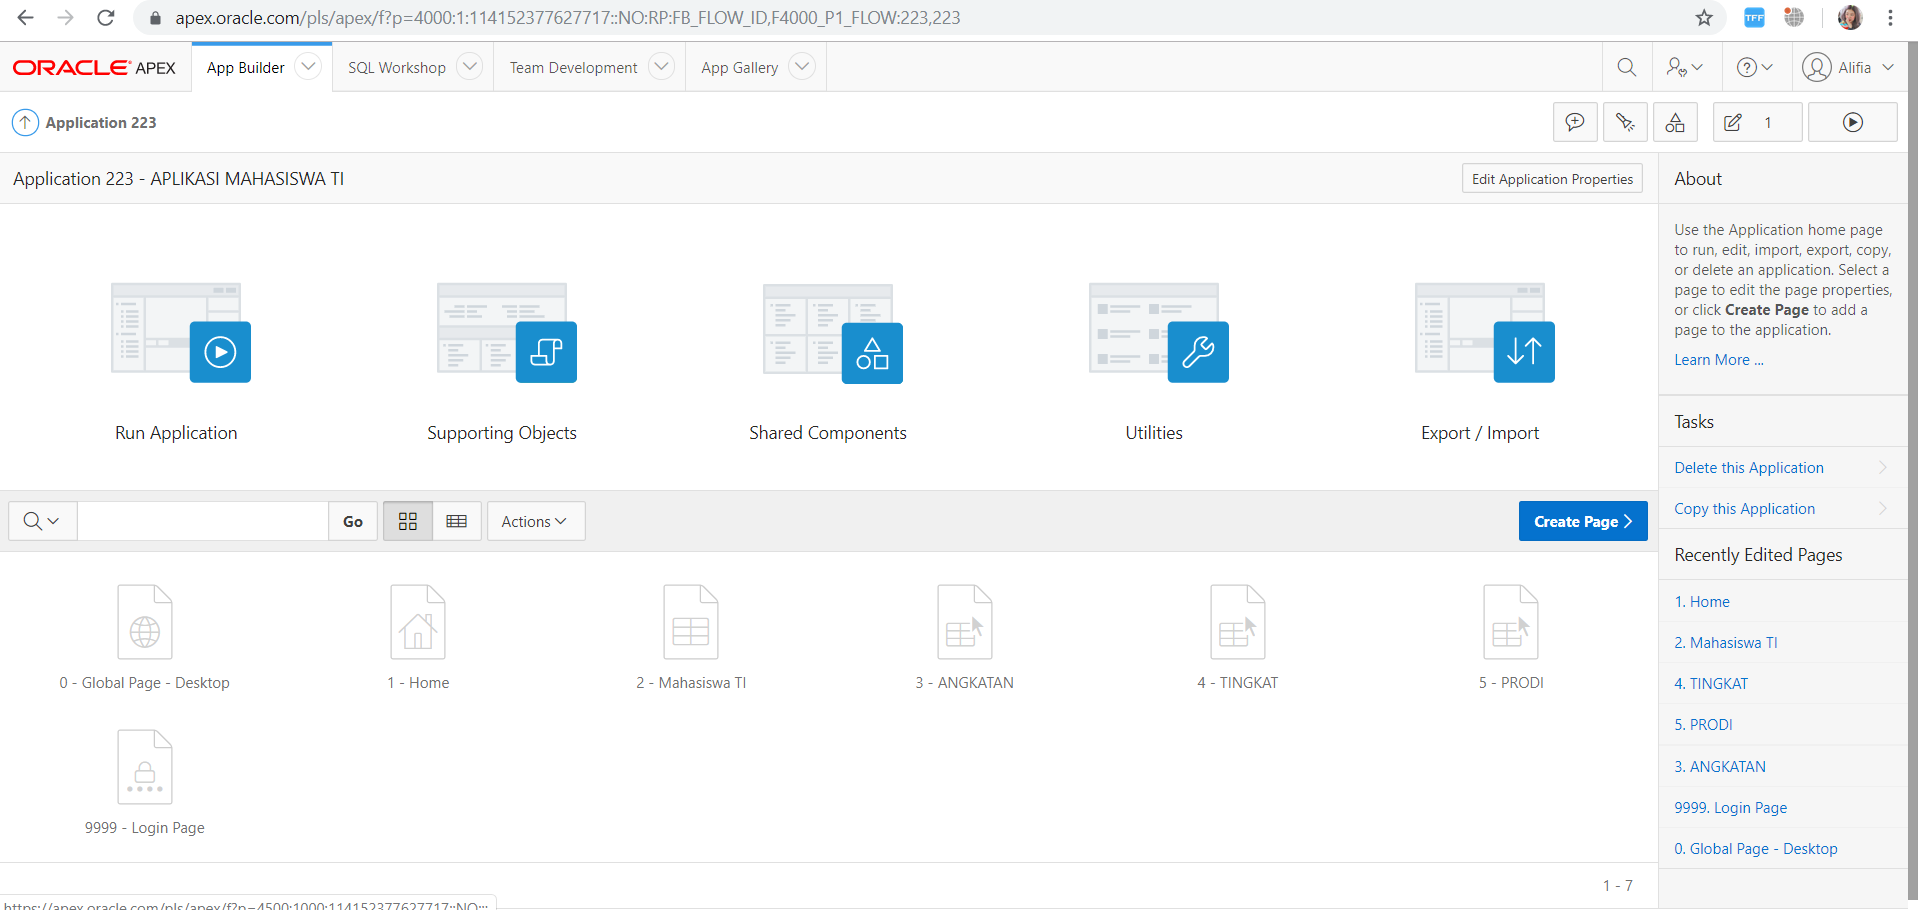
\includegraphics[width=8cm]{GAMBAR/RUNAPPLICATION.PNG}}
        \end{figure}
    \item Selesai, aplikasi anda telah dibuat.
        \begin{figure}[h]
        \centerline{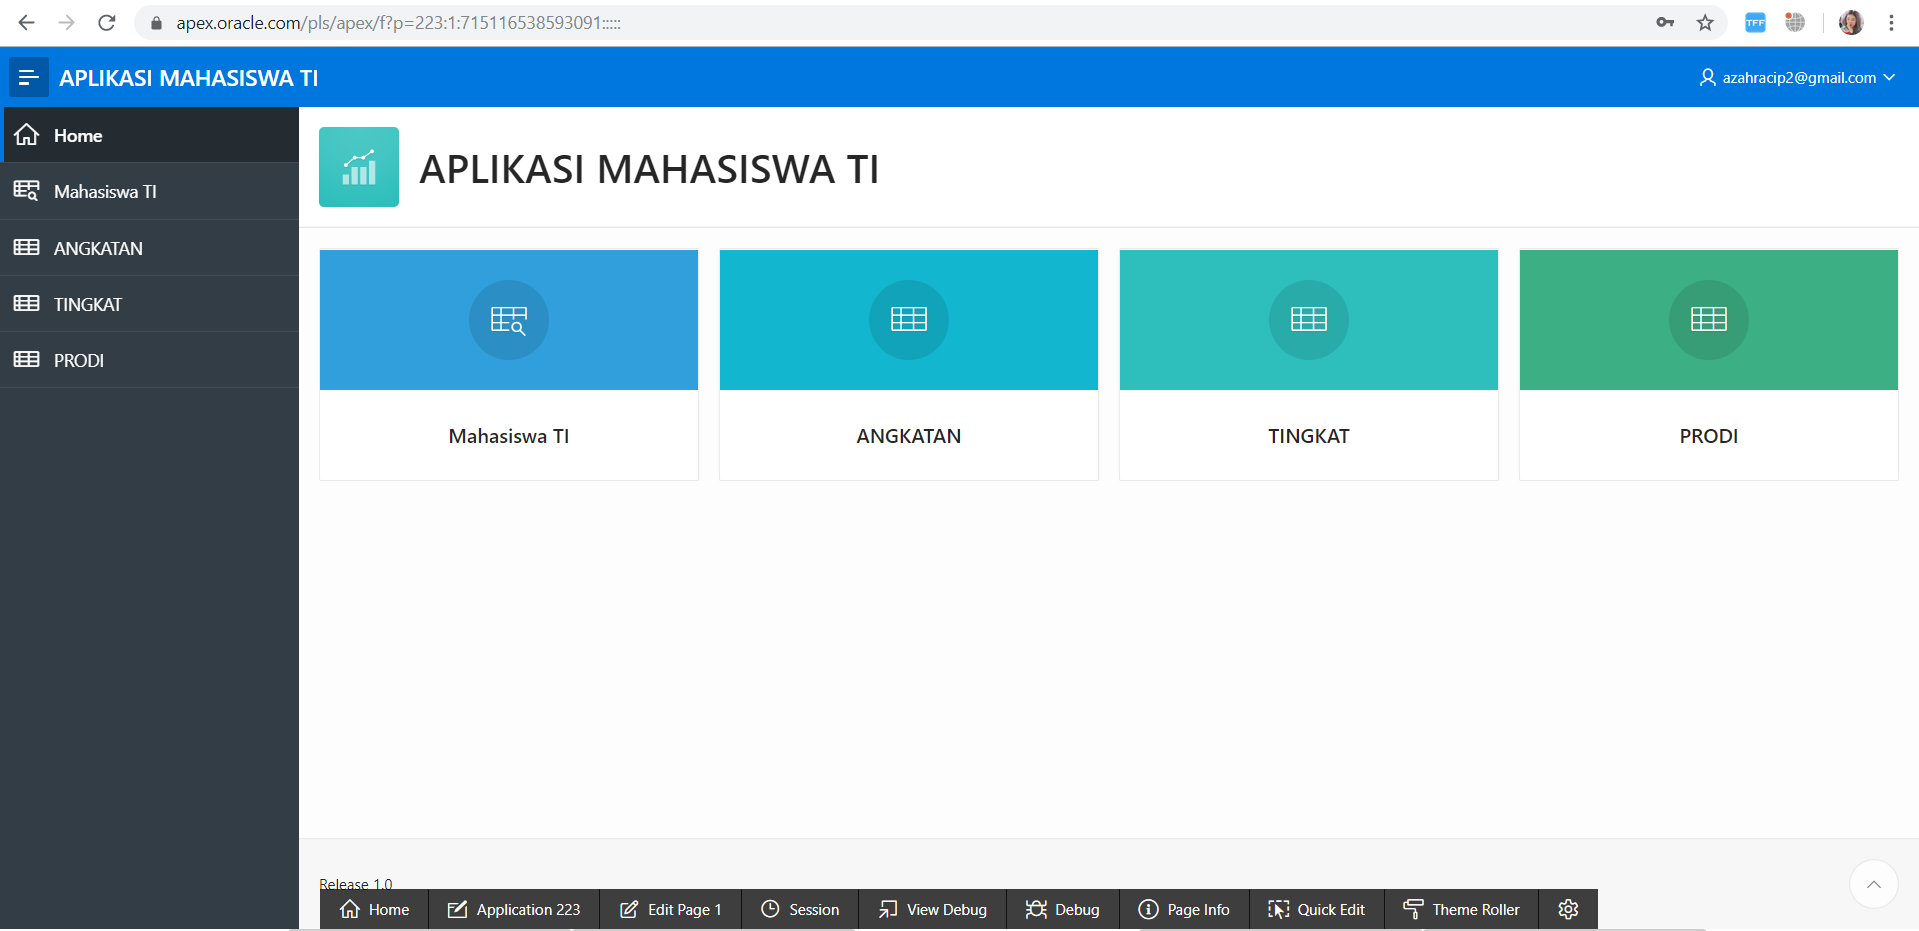
\includegraphics[width=8cm]{GAMBAR/tampilan.PNG}}
        \end{figure}
    
    
    
    
    
    
    
\end{enumerate}